\nocite{srssbrs} % Sequential/Session-based Recommendations: Challenges, Approaches, Applications and Opportunities

\section*{Introdução}

Esse projeto tem como propósito a produção de um material didático
sobre sistemas de recomendação sequenciais.
O objetivo é apresentar uma visão geral sobre o assunto, enquanto
apresentamos uma abordagem de implementação de sistemas de recomendação
sequenciais baseada em  redes neurais de atenção e um modelo baseado em 
fatoração de matrizes com cadeias de Markov.

\section*{Metodologia}

Para esse projeto, iremos utilizar dois algoritmos de recomendação:
o \textit{Self-Attentive Sequential Recommendation (SASRec)} \cite{sasrec} e
o \textit{Factorizing Personalized Markov Chains (FPMC)} \cite{fpmc}.
O SASRec é um algoritmo proposto por Wang-Cheng Kang e Julian McAuley em 2018
consiste em uma rede neural de atenção que é treinada para prever o
próximo item a ser recomendado em uma recomendação sequencial. Já o FPMC é
um algoritmo proposto por Rendle, Freudenthaler e Schmidt-Thieme em 2010
e consiste de uma abordagem híbrida baseando-se na ideia de fatoração de 
matrizes e cadeias de markov junto a técnica BPR (Bayesian Personalized Ranking)
para prever a próxima "cesta" (uma única música no nosso contexto) a ser 
recomendada a partir da "cesta" anterior.

Além disso, iremos utilizar o dataset de reproduções de músicas
do site \url{last.fm} disponível em \citeurl{lastfm_dataset}
\cite{lastfm_dataset} por \citeauthor{lastfm_book} \cite{lastfm_book}.

Esse dataset de 2010 apresenta o histórico de reprodução de músicas
de uma amostra de 1.000 usuários. Pela natureza do \url{last.fm},
cada usuário tem em média aproximadamente 20 mil reproduções de músicas,
resultando em um total de aproximadamente 19 milhões de reproduções
de músicas no dataset.

Produzimos dois notebooks disponíveis em
\url{https://github.com/LiviaLelis/recsys-tp-seq}, junto ao material textual do
projeto e instruções de uso. Todo o material e explicações estão disponíveis
pelos próprios notebooks.

Além disso, foi produzida uma vídeo aula explicativa sobre sistemas de
% TODO: Adicionar link
recomendação sequencial disponível em \url{https://youtu.be/3-4-5-6},
para dar uma breve introdução ao assunto e apresentar as implementações
feitas neste projeto.

Esse material então foi enviado para algumas pessoal que atuam com 
conhecimento técnico na área de computação junto a um formulário de
avaliação de projeto para medir a qualidade do trabalho produzido.

\section*{Implementação}

\subsection*{Dataset}

Para o dataset, fizemos algumas modificações para adequar-se
as necessidades do algoritmo. Primeiramente, fizemos um
mapeamento dos UUIDs (universally unique identifier) para inteiros
sequenciais a partir do 1, já que necessitamos de representações
numéricas para os algoritmos.

Além disso, devido à natureza do \url{last.fm}, cada usuário tem
um volume extenso de reproduções de músicas. Entendemos que esse
histórico extenso pode ser dívido em "sessões de reprodução", 
isto é, um conjunto de reproduções de músicas que ocorrem de 
maneira quase contínua no tempo. Portanto, para cada usuário,
construímos um conjunto de sessões, tomando como critério para
uma sessão a reprodução de músicas que ocorrem em um intervalo
máximo de 30 minutos entre duas reproduções consecutivas. Acreditamos
que essa abordagem de tratamento de dados seja mais adequada para
o problema, reduzindo o tamanho das sequências e mantendo-as mais
coerentes, já que as preferências musicais de um usuário pode variar
entre sessões e com o tempo, entretanto não conseguimos medir se
essa assunção é verdadeira.

\subsection*{Modelo de Atenção}

O SASRec \cite{sasrec} é um modelo lançado em 2018 e foi um dos primeiros 
algoritmos de recomendação sequencial baseado na técnica de \textit{self-attention}
introduzida introduzida no artigo \citetitle{attetionisallyouneed} 
\cite{attetionisallyouneed}, sendo o SASRec um dos pioneiros trazendo essa ideia
para o campo de sistemas de recomendação sequenciais.

\begin{figure}[H]
    \centering
    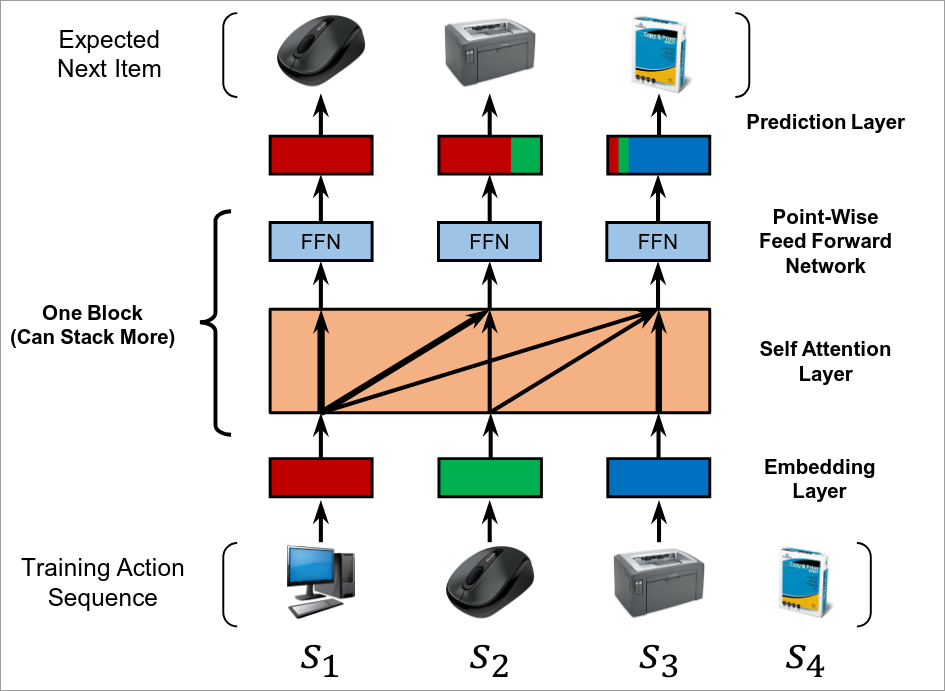
\includegraphics[width=0.6\textwidth]{../assets/sasrec-diagram.png}
    \caption{Diagrama da arquitetura do modelo SASRec \cite{sasrec}}
    \label{fig:sasrec-diagram}
\end{figure}

Nossa implementação é baseada em uma adaptação \cite{seanswyi} em
PyTorch do modelo dos autores originais implementado em TensorFlow.
Nessa adaptação, não fizemos mudanças diretas na arquitetura do
modelo, mas apenas algumas adaptações de código para melhorar a
legibilidade e o desempenho. Além disso, desviamos da implementação original 
nos parâmetros escolhidos, otimizador e outras configurações.

A versão final do modelo foi treinada com uma amostra aleatória
de 100 mil sessões para reduzir o tempo de treinamento ao custo
de uma perda potencialmente pequena de qualidade. Além disso,
para a divisão dos dados, fizemos uma divisão de treino, teste
e validação pela estratégia sugerida pelos autores de truncamento
das sessões, isto é, todas as divisões contêm todas as sessões,
sendo que na divisão de treino é descartada os dois últimos itens
da sessão, na de validação o último item da sessão e na de teste
é mantida a sessão inteira. Como nosso volume de dados era
suficientemente grande, acreditamos que poderíamos obter resultados
mais realistas se seguíssemos uma divisão por meio das sessões em
si ao invés deste truncamento.

Além disso, para melhorar a performance do modelo e viabilizar o treinamento,
é adotada a estratégia original de construção de amostras negativas, isto é,
geramos para cada item um conjunto de itens negativos para que o
treinamento seja mais eficiente, realizando uma classificação
binária de se o item é positivo ou negativo.

A função de perda utilizada para avaliar o modelo foi a 
\textit{Binary Cross Entropy with Logits}, que é uma função de perda
para classificação binária. Além disso fizemos uso do algoritmo
de otimização AdamW \cite{adamw} com o parâmetro de learning rate
fixo. Também fizemos experimentos com o \textit{scheduler OneCycleLR} 
\cite{onecyclelr} que apresentou resultados bem semelhantes, por isso
seguimos com a learning rate fixa para deixar os resultados mais comparáveis.

Mais informações sobre os parâmetros escolhidos podem ser vistas
no repositório do projeto disponível em \url{https://github.com/LiviaLelis/recsys-tp-seq}.

\subsection{FPMC}

O FPMC \cite{fpmc} é um modelo lançado em 2010 que combina a técnica de 
fatoração de matrizes (usando BPR) com a técnica de cadeias de Markov.

\begin{figure}[H]
    \centering
    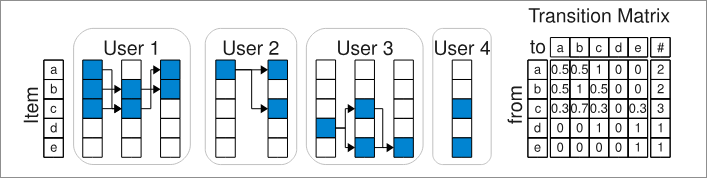
\includegraphics[width=0.6\textwidth]{../assets/fpmc-diagram.png}
    \caption{Diagrama da arquitetura do modelo FPMC \cite{fpmc}}
    \label{fig:fpmc-diagram}
\end{figure}

A implementação do modelo FPMC é bem simples, se diferenciando principalmente
pelo uso da BPR como função de perda. Além disso, a estrutura dos dados
consumidos pelo modelo é distinta, tomando como entrada uma lista de tuplas
do tipo (usuário, item anterior, próximo item real, próximo item negativo 
[gerado no dataset]), ou seja, diferentemente do modelo SASRec, o usuário é
levado em consideração, mas, ao invés de tomar como entrada uma lista de 
itens, recebe apenas o item anterior.

\section*{Resultados}

A fim de melhor comparar os dois modelos, optamos por em ambos utilizar a mesma
amostra de 100k sessões para reduzir o tempo de treinamento ao custo de uma
redução na qualidade da base de dados. Além disso, as condições de treinamento
foram definidas mantendo parâmetros semelhantes: ambos com um \textit{batch size}
de 1024 e sem scheduler. Além disso, foi selecionado um número de epochs para 
manter ambos tempos de treinamento próximos (aproximadamente 40 minutos em uma
RTX 3080TI).

% Criar uma tabela onde as colunas são o modelo e as linhas as métricas

\begin{table}[H]
    \centering
    \begin{tabular}{|c|c|c|c|}
        \hline
        Modelo & NDCG@10 & HIT@10 \\ \hline
        SASRec & 0.6757 & 0.7704 \\ \hline
        FPMC & 0.6733 & 0.7437 \\ \hline
    \end{tabular}
    \caption{Métricas de qualidade do SASRec e FPMC nos dados de teste}
    \label{tab:results}
\end{table}

Ambos os modelos apresentam resultados muito parecidos, com o SASRec tomando uma
leve margem de melhoria. Ambos os modelos ainda apresentam potencial de melhoria
já que nenhum deles paracia ter convergido completamente durante o treinamento,
além da possibilidade de tunar os hiperparâmetros de treinamento.

Desse modo, não é possível declarar um modelo como claramente superior ao outro,
porém o FPMC costuma ser menos custoso e convergir mais rapidamente que o SASRec,
sendo uma boa alternativa para situações onde é necessário reduzir o custo de
treinamento ao mesmo tempo que se mantém um bom resultado.

No artigo original do modelo SASRec \cite{sasrec}, ele supera o FPMC em
todos os datasets utilizados (que não incluem o utilizado aqui), mas também em
uma margem de melhoria moderada (mas mais significativa do que as apresentadas
aqui).

\section*{Avaliação do material}

TODO :)
